\chapter{Superposition d'une couche fluide sur une couche poreuse}

Dans ce chapitre, on essaie d'étudier les nouvelles conditions de saut pour les problèmes d'écoulement fluide avec interface avec un milieu poreux. La modélisation, en particulier la dérivation des conditions de saut et leur comparaison avec d'autres jeux de conditions ont été traités dans \cite{angot:hal-01583856}. L'analyse du système couplé se trouve par exemple dans \cite{angot:hal-01635289}. 

\section{Mise en situation}

Soit $\Omega$ un ouvert connexe borné de $\mathbb{R}^d$ avec $d \leqslant 3$. On suppose que sa frontière $\Gamma := \partial \Omega$ est lipschitzienne et on note $\mathbf{\nu}$ le vecteur unitaire sortant de ce domaine. Le domaine $\Omega$ est divisé en deux composantes connexes disjointes $\Omega_f$, région fluide, $\Omega_p$, région poreuse, séparées par une frontière lipschitzienne commune $\Sigma \subset \mathbb{R}^{d-1}$. L'hyperplan $\Sigma$ est muni d'une base orthonormée $\{\tau_j\}$, $j \leqslant d-1$ et d'un vecteur normal $\mathbf{n}$ dont on fixe le sens comme étant de la région poreuse vers la région fluide. La situation se résume par le dessin, issu de \cite{angot:hal-03172378}, figure 1 :
\begin{figure}[htp]
    \centering
    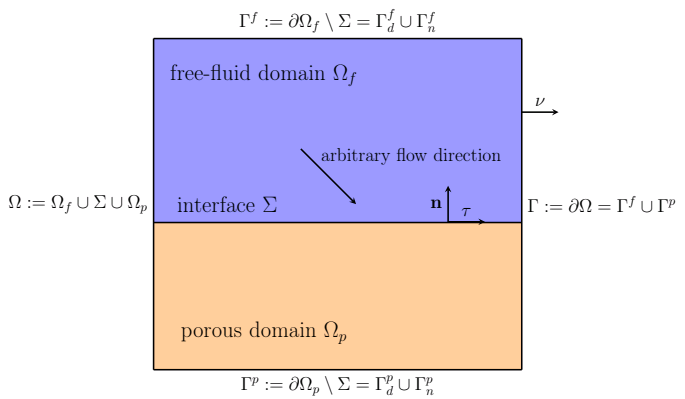
\includegraphics[width=15cm]{Images/bicouche/situation.png}
    \caption{Situation ; $\Gamma^p_d$ et $\Gamma^f_d$ sont munis de conditions de Dirichlet en vitesse et $\Gamma^p_n$ ou $\Gamma^f_n$ sont munies de conditions de Neumann, en vitesse également.}
    \label{fig:bicouche}
\end{figure}

Les auteurs introduisent alors le cadre fonctionnel. On notera $H^{s}(\Omega) := W^{s, 2}(\Omega)$, muni des normes usuelles
$$ \| u \|_{s, \Omega} := \int_{\Omega} (1 + |\xi|^2)^s |\hat{u}(\xi)|^2 d\xi $$

On note $ < \cdot, \cdot >_{-1, \Omega}$ le crochet de dualité entre $H^{-1}(\Omega)$ et $H^{1}_{0}(\Omega)$. On introduit enfin les espaces de Hilbert réels $$ \mathbf{H}_{div}(\Omega) := \{ u \in L^2(\Omega) ; \nabla \cdot u \in L^2(\Omega) \} $$ muni de la norme de graphe définie par $$ \| u \|^2_{\mathbf{H}_{div}} := \| u \|^2_{0, \Omega} + \| \nabla \cdot u \|^2_{0, \Omega} $$ et $$ L^2_0(\Omega) := \{ q \in L^2(\Omega) ; \int_{\Omega} q(x) dx = 0 \} $$ muni de la norme usuelle $\| \cdot \|_{0, \Omega}$.

Le cadre fonctionnel propre à $\Sigma$ est ensuite introduit. Il est question des espaces $\tilde{H}^{1/2}(\Sigma)$ l'espace des traces des fonctions $H^1_{0, \partial \Omega_f \backslash \Sigma}$ ou $H^1_{0, \partial \Omega_p \backslash \Sigma}$, nulles sur les bords $\partial \Omega_f \backslash \Sigma$ ou $\partial \Omega_p \backslash \Sigma$. Ils notent de plus $< \cdot, \cdot >_{-1/2, \Sigma}$ le crochet de dualité entre $\tilde{H}^{-1/2}(\Sigma)$ et $\tilde{H}^{1/2}(\Sigma)$. L'espace $\tilde{H}^{-1/2}(\Sigma)$ étant un espace de distributions sur $\Sigma$. Les deux espaces $H^{1/2}(\Sigma)$ et $\tilde{H}^{1/2}(\Sigma)$ sont équipés des normes
\begin{align*}
    |u|^2_{H^{1/2}(\Sigma)} := \int_{\Sigma} \int_{\Sigma} \frac{|u(\mathbf{x}) - u(\mathbf{y}|^2}{|\mathbf{y} - \mathbf{x}|^d} d\mathbf{x} d\mathbf{y} & \hspace{7.5pt} ; \hspace{7.5pt} \| u \|^2_{H^{1/2}(\Sigma)} := \| u \|^2_{0, \Sigma} + | \nabla u |^2_{H^{1/2}(\Sigma)} \\
    |u|^2_{\tilde{H}^{1/2}(\Sigma)} := |u|^2_{H^{1/2}(\Sigma)} + \int_{\Sigma} \frac{|u(\mathbf{x})|^2}{d(\mathbf{x}, \partial \Sigma)} d\mathbf{x} & \hspace{7.5pt} ; \hspace{7.5pt} \| u \|^2_{\tilde{H}^{1/2}(\Sigma)} := \| u \|^2_{0, \Sigma} + | u |^2_{\tilde{H}^{1/2}(\Sigma)}
\end{align*}
où $d(\mathbf{x}, \partial \Sigma) := \inf\{ d(\mathbf{x}, \mathbf{y}) ; \mathbf{y} \in \partial \Sigma \}$. L'écriture des normes est licite du fait qu'on a les injections $$ H^{1/2}(\Sigma) \hookrightarrow L^2(\Sigma) $$ et $$ \tilde{H}^{1/2}(\Sigma) \hookrightarrow L^2(\Sigma) $$ En guise de propriétés, sont cités le fait que l'injection de $\tilde{H}^{1/2}(\Sigma) \hookrightarrow H^{1/2}(\Sigma)$ est continue du fait que la distance de $d(\mathbf{x}, \partial \Sigma)$ est $W^{1, \infty}(\Sigma)$ mais l'équivalence entre les normes n'est vaie que si $\Sigma$ est une courbe fermée lorsque $d=2$ ou plus généralement une surface fermée. Enfin, les auteurs proposent la propriété suivante pour les prolongements par $0$ de fonctions $\tilde{u} \in \tilde{H}^{1/2}(\Sigma)$ à tout $\partial \Omega_f$ (respectivement $\partial \Omega_p$), noté $u \in H^{1/2}(\partial \Omega_f)$ : $$ \exists c(\Sigma, \partial \Omega_f) > 0 \hspace{10pt} \forall \tilde{u} \in \tilde{H}^{1/2}(\Sigma) \hspace{15pt} \| u \|_{H}^{1/2}(\Sigma) \leqslant c(\Sigma, \partial \Omega_f) \| u \|_{\tilde{H}^{1/2}(\Sigma)} $$

\paragraph{Modèle pour le milieu fluide $\Omega_f$} Dans la région purement fluide, on considère le modèle de Stokes à masse volumique et viscosité constantes, qui correspond à un écoulement incompressible d'un fluide visqueux à faible nombre de Reynolds
\begin{equation*}
\begin{array}{rr}
    \nabla \cdot \mathbf{v} = 0 & (0, T) \times \Omega_f \\
    \rho \partial_t \mathbf{v} - \mu \nabla \left(\nabla \mathbf{v} + \nabla \mathbf{v}^T\right) + \nabla p = \rho \mathbf{f^f} & (0, T) \times \Omega_f
\end{array}
\end{equation*}

\paragraph{Modèle pour le milieu poreux} On regarde dans le milieu poreux le problème de Brinkman pour un fluide visqueux incompressible s'écoulant à faible nombre de Reynolds.
\begin{equation*}
\begin{array}{rr}
    \nabla \cdot \mathbf{v} = 0 & (0, T) \times \Omega_p \\
    \frac{\rho}{\phi} \partial_t \mathbf{v} - \frac{\mu}{\phi} \nabla \left(\nabla \mathbf{v} + \nabla \mathbf{v}^T\right) + \mu \mathbf{K}^{-1} + \nabla p = \rho \mathbf{f^p} & (0, T) \times \Omega_p
\end{array}
\end{equation*}

\paragraph{Tenseur de stress du problème} Pour la région fluide, on introduit le tenseur de Cauchy du milieu $$ \sigma^f(\mathbf{v}, p) := \mu \left( \nabla \mathbf{v} + \nabla \mathbf{v}^T \right) - p \text{Id}_{\mathbb{R}^d} $$ et dans la région poreuse le tenseur $$ \sigma^p(\mathbf{v}, p) := \frac{\mu}{\phi} \left( \nabla \mathbf{v} + \mathbf{v}^T) \right) - p \text{Id}_{\mathbb{R}^d} $$

\paragraph{Existence et unicité avec viscosité variable} Pour l'analyse du système dans son cas le plus général, on se référera à \cite{angot:hal-01635289}.

\section{Expérience numérique en 2.D}

La seule expérience à laquelle je me serai prêté est la suivante : essayer de simuler le tourbillon de Taylor-Green, avec un saut nul sur la vitesse comme sur la pression. Des solutions de Taylor-Green, on explicite le problème avec les deux sauts nuls. L'idée étant de tester plusieurs altitudes pour la surface $\Sigma$, comme présentée dans \cite{angot:hal-03172378}. Au cours du stage, je n'aurai eu le temps que d'effectuer une simulation, qui est présentée ici.

On implémente le système couplé à partir des solutions de Taylor-Green. Le saut en pression comme en vitesse est nul. Le champ de divergence est nul en tout temps et en tout point ; on suppose que l'interface porte une densité de force nulle. Le système, pour Taylor-Green, s'écrit, avec tenseur de perméabilité réduit à un scalaire :
\begin{align*}
    \partial_x u + \partial_y = & 0 \hspace{15pt} & \Omega \\
    -\partial_t u - \Delta u + \partial_x p = & 0 \hspace{15pt} &  \Omega^f \\
    -\frac{1}{\phi}\partial_t u - \frac{1}{\phi} \Delta u + \frac{1}{K} u = & \frac{1}{K} u \hspace{15pt} & \Omega^p \\
    -\partial_t v - \Delta v + \partial_y p = & 0 \hspace{15pt} & \Omega^f \\
    -\frac{1}{\phi}\partial_t v - \frac{1}{\phi} \Delta v + \frac{1}{K} v + \partial_y p = & \frac{1}{K} v \hspace{15pt} & \Omega^p
\end{align*}
Fixant $\Sigma$ au milieu du domaine, sur une ligne de pression / vitesse horizontale, l'idée était d'assembler le système par région. On note $n_y$ (un nombre pair) le nombre de volumes sur la dimension verticale, on compte donc $n_y/2$ volumes dans la région fluide et $n_y/2$ dans la région poreuse.

\begin{minted}{python}
# Assemblage du prédicteur sur la vitesse U
N = 5*(ny-1)*nx + 2*(ny-1) + 2*(nx+2)
lignes   = numpy.zeros(N)
colonnes = numpy.zeros(N)
donnees  = numpy.zeros(N)

compteur = 0
    for j in range(ny+1):
        for i in range(nx+2):
        
            # Si U[j,i] est au bord, appliquer la condition de Dirichlet
            if i == 0 or i == nx+1 or j == 0 or j == ny:
                lignes[compteur]   = j * (nx+2) + i
                colonnes[compteur] = j * (nx+2) + i
                donnees[compteur]  = 1
                compteur += 1
            
            # U[j,1] dans le milieu poreux (Brinkman)
            elif i == 1 and j < ny//2:
                lignes[compteur : compteur+5] = j * (nx+2) + i
                colonnes[compteur]   = j * (nx+2) + i
                colonnes[compteur+1] = j * (nx+2) + i - 1
                colonnes[compteur+2] = j * (nx+2) + i + 1
                colonnes[compteur+3] = (j-1) * (nx+2) + i
                colonnes[compteur+4] = (j+1) * (nx+2) + i
                donnees[compteur]    = mu/phi*(3*(dy/dx) + 2*(dx/dy)) + (dy*dx)/dt + (dy*dx)*mu/Kp
                donnees[compteur+1]  = mu/phi*(-2*dy/dx)
                donnees[compteur+2]  = mu/phi*(-dy/dx)
                donnees[compteur+3]  = mu/phi*(-dx/dy)
                donnees[compteur+4]  = mu/phi*(-dx/dy)
                compteur += 5
        
            # U[j,1] dans le milieu fluide (Stokes)
            elif i == 1 and j > ny//2-1:
                lignes[compteur : compteur+5] = j * (nx+2) + i
                colonnes[compteur]   = j * (nx+2) + i
                colonnes[compteur+1] = j * (nx+2) + i - 1
                colonnes[compteur+2] = j * (nx+2) + i + 1
                colonnes[compteur+3] = (j-1) * (nx+2) + i
                colonnes[compteur+4] = (j+1) * (nx+2) + i
                donnees[compteur]    = mu*(3*(dy/dx) + 2*(dx/dy)) + + (dy*dx)/dt
                donnees[compteur+1]  = mu*(-2*dy/dx)
                donnees[compteur+2]  = mu*(-dy/dx)
                donnees[compteur+3]  = mu*(-dx/dy)
                donnees[compteur+4]  = mu*(-dx/dy)
                compteur += 5
            
            # U[j,nx] dans le milieu poreux (Brinkman)
            elif i == nx and j < ny//2:
                lignes[compteur : compteur+5] = j * (nx+2) + i
                colonnes[compteur]   = j * (nx+2) + i
                colonnes[compteur+1] = j * (nx+2) + i - 1
                colonnes[compteur+2] = j * (nx+2) + i + 1
                colonnes[compteur+3] = (j-1) * (nx+2) + i
                colonnes[compteur+4] = (j+1) * (nx+2) + i
                donnees[compteur]    = mu/phi*(3*(dy/dx) + 2*(dx/dy)) + (dy*dx)/dt + (dy*dx)*mu/Kp
                donnees[compteur+1]  = mu/phi*(-dy/dx)
                donnees[compteur+2]  = mu/phi*(-2*dy/dx)
                donnees[compteur+3]  = mu/phi*(-dx/dy)
                donnees[compteur+4]  = mu/phi*(-dx/dy)
                compteur += 5
        
            # U[j,nx] dans le milieu fluide (Stokes)
            elif i == nx and j > ny//2-1:
                lignes[compteur : compteur+5] = j * (nx+2) + i
                colonnes[compteur]   = j * (nx+2) + i
                colonnes[compteur+1] = j * (nx+2) + i - 1
                colonnes[compteur+2] = j * (nx+2) + i + 1
                colonnes[compteur+3] = (j-1) * (nx+2) + i
                colonnes[compteur+4] = (j+1) * (nx+2) + i
                donnees[compteur]    = mu*(3*(dy/dx) + 2*(dx/dy)) + (dy*dx)/dt
                donnees[compteur+1]  = mu*(-dy/dx)
                donnees[compteur+2]  = mu*(-2*dy/dx)
                donnees[compteur+3]  = mu*(-dx/dy)
                donnees[compteur+4]  = mu*(-dx/dy)
                compteur += 5
            
            # U[j,i] à l'intérieur de la région poreuse (Brinkman)
            elif j < ny//2:
                lignes[compteur : compteur+5] = j * (nx+2) + i
                colonnes[compteur]   = j * (nx+2) + i
                colonnes[compteur+1] = j * (nx+2) + i - 1
                colonnes[compteur+2] = j * (nx+2) + i + 1
                colonnes[compteur+3] = (j-1) * (nx+2) + i
                colonnes[compteur+4] = (j+1) * (nx+2) + i
                donnees[compteur]    = mu/phi*(2 * (dy/dx + dx/dy)) + (dy*dx)/dt + (dy*dx)*mu/Kp
                donnees[compteur+1]  = mu/phi*(-dy/dx)
                donnees[compteur+2]  = mu/phi*(-dy/dx)
                donnees[compteur+3]  = mu/phi*(-dx/dy)
                donnees[compteur+4]  = mu/phi*(-dx/dy)
                compteur += 5
        
            # U[j,i] à l'intérieur de la région fluide (Stokes)
            else:
                lignes[compteur : compteur+5] = j * (nx+2) + i
                colonnes[compteur]   = j * (nx+2) + i
                colonnes[compteur+1] = j * (nx+2) + i - 1
                colonnes[compteur+2] = j * (nx+2) + i + 1
                colonnes[compteur+3] = (j-1) * (nx+2) + i
                colonnes[compteur+4] = (j+1) * (nx+2) + i
                donnees[compteur]    = mu*(2 * (dy/dx + dx/dy)) + (dy*dx)/dt
                donnees[compteur+1]  = mu*(-dy/dx)
                donnees[compteur+2]  = mu*(-dy/dx)
                donnees[compteur+3]  = mu*(-dx/dy)
                donnees[compteur+4]  = mu*(-dx/dy)
                compteur += 5

Auu = sparse.coo_matrix((donnees, (lignes, colonnes)), shape=((ny+1)*(nx+2), (ny+1)*(nx+2))).tocsc()
Mu = sparse.linalg.LinearOperator(((ny+1)*(nx+2), (ny+1)*(nx+2)), splu(Auu).solve)
\end{minted}

\begin{minted}{python}
# Assemblage du prédicteur sur la vitesse V
N = 5*ny*(nx-1) + 2*(ny+2) + 2*(nx-1)
lignes   = numpy.zeros(N)
colonnes = numpy.zeros(N)
donnees  = numpy.zeros(N)

compteur = 0
for j in range(ny+2):
    for i in range(nx+1):
        
        # Si V[j,i] est sur le bord du domaine
        if i == 0 or i == nx or j == 0 or j == ny+1:
            lignes[compteur]   = j * (nx+1) + i
            colonnes[compteur] = j * (nx+1) + i
            donnees[compteur]  = 1
            compteur += 1
                
        # Si V[j,i] est sur la deuxième ligne (Brinkman)
        elif j == 1:
            lignes[compteur : compteur+5] = j * (nx+1) + i
            colonnes[compteur]   = j * (nx+1) + i
            colonnes[compteur+1] = j * (nx+1) + i - 1
            colonnes[compteur+2] = j * (nx+1) + i + 1
            colonnes[compteur+3] = (j-1) * (nx+1) + i
            colonnes[compteur+4] = (j+1) * (nx+1) + i
            donnees[compteur]    = mu/phi*(2*(dy/dx) + 3*(dx/dy)) + (dy*dx)/dt + (dy*dx)*mu/Kp
            donnees[compteur+1]  = mu/phi*(-dy/dx)
            donnees[compteur+2]  = mu/phi*(-dy/dx)
            donnees[compteur+3]  = mu/phi*(-2 * dx/dy)
            donnees[compteur+4]  = mu/phi*(-dx/dy)
            compteur += 5
        
        # Si V[j,i] est sur l'avant-dernière ligne (Stokes)
        elif j == ny:
            lignes[compteur : compteur+5] = j * (nx+1) + i
            colonnes[compteur]   = j * (nx+1) + i
            colonnes[compteur+1] = j * (nx+1) + i - 1
            colonnes[compteur+2] = j * (nx+1) + i + 1
            colonnes[compteur+3] = (j-1) * (nx+1) + i
            colonnes[compteur+4] = (j+1) * (nx+1) + i
            donnees[compteur]    = mu*(2*(dy/dx) + 3*(dx/dy)) + (dy*dx)/dt
            donnees[compteur+1]  = mu*(-dy/dx)
            donnees[compteur+2]  = mu*(-dy/dx)
            donnees[compteur+3]  = mu*(-dx/dy)
            donnees[compteur+4]  = mu*(-2 * dx/dy)
            compteur += 5
        
        # Si V[j,i] est à l'intérieur de la région poreuse (Brinkman)
        elif j < ny//2:
            lignes[compteur : compteur+5] = j * (nx+1) + i
            colonnes[compteur]   = j * (nx+1) + i
            colonnes[compteur+1] = j * (nx+1) + i - 1
            colonnes[compteur+2] = j * (nx+1) + i + 1
            colonnes[compteur+3] = (j-1) * (nx+1) + i
            colonnes[compteur+4] = (j+1) * (nx+1) + i
            donnees[compteur]    = mu/phi*(2 * (dy/dx + dx/dy)) + (dy*dx)/dt + (dy*dx)*mu/Kp
            donnees[compteur+1]  = mu/phi*(-dy/dx)
            donnees[compteur+2]  = mu/phi*(-dy/dx)
            donnees[compteur+3]  = mu/phi*(-dx/dy)
            donnees[compteur+4]  = mu/phi*(-dx/dy)
            compteur += 5
        
        # Si V[j,i] est à l'intérieur de la région fluide (Stokes)
        elif j > ny//2-1:
            lignes[compteur : compteur+5] = j * (nx+1) + i
            colonnes[compteur]   = j * (nx+1) + i
            colonnes[compteur+1] = j * (nx+1) + i - 1
            colonnes[compteur+2] = j * (nx+1) + i + 1
            colonnes[compteur+3] = (j-1) * (nx+1) + i
            colonnes[compteur+4] = (j+1) * (nx+1) + i
            donnees[compteur]    = mu*(2 * (dy/dx + dx/dy)) + (dy*dx)/dt
            donnees[compteur+1]  = mu*(-dy/dx)
            donnees[compteur+2]  = mu*(-dy/dx)
            donnees[compteur+3]  = mu*(-dx/dy)
            donnees[compteur+4]  = mu*(-dx/dy)
            compteur += 5
        
Avv = sparse.coo_matrix((donnees, (lignes, colonnes)), shape=((ny+2)*(nx+1), (ny+2)*(nx+1))).tocsc()
Mv = sparse.linalg.LinearOperator(((ny+2)*(nx+1), (ny+2)*(nx+1)), splu(Avv).solve)
\end{minted}
       
\begin{minted}{python}
# Assemblage du Laplacien de Neumann pour P
N = 5*(ny-1)*(nx-1) + 2*4*(ny-1) + 2*4*(nx-1) + 3 * 3 + 1
lignes   = numpy.zeros(N)
colonnes = numpy.zeros(N)
donnees  = numpy.zeros(N)

compteur = 0
for j in range(ny+1):
        for i in range(nx+1):
        
            if i == 0 and j == 0:
                lignes[compteur]   = j * (nx+1) + i
                colonnes[compteur] = j * (nx+1) + i
                donnees[compteur]  = 1
                compteur += 1
        
            elif i == 0 and j == ny:
                lignes[compteur : compteur+3] = j * (nx+1) + i
                colonnes[compteur]   = j * (nx+1) + i
                colonnes[compteur+1] = j * (nx+1) + i + 1
                colonnes[compteur+2] = (j-1) * (nx+1) + i
                donnees[compteur]    = - 2 * (dy/dx + dx/dy)
                donnees[compteur+1]  = 2 * dy / dx
                donnees[compteur+2]  = 2 * dx / dy
                compteur += 3
            
            elif i == nx and j == 0:
                lignes[compteur : compteur+3] = j * (nx+1) + i
                colonnes[compteur]   = j * (nx+1) + i
                colonnes[compteur+1] = j * (nx+1) + i - 1
                colonnes[compteur+2] = (j+1) * (nx+1) + i
                donnees[compteur]    = - 2 * (dy/dx + dx/dy)
                donnees[compteur+1]  = 2 * dy / dx
                donnees[compteur+2]  = 2 * dx / dy
                compteur += 3

            elif i == nx and j == ny:
                lignes[compteur : compteur+3] = j * (nx+1) + i
                colonnes[compteur]   = j * (nx+1) + i
                colonnes[compteur+1] = j * (nx+1) + i - 1
                colonnes[compteur+2] = (j-1) * (nx+1) + i
                donnees[compteur]    = - 2 * (dy/dx + dx/dy)
                donnees[compteur+1]  = 2 * dy / dx
                donnees[compteur+2]  = 2 * dx / dy
                compteur += 3
    
            elif i == 0 and j > 0 and j < ny:
                lignes[compteur : compteur+4] = j * (nx+1) + i
                colonnes[compteur]   = j * (nx+1) + i
                colonnes[compteur+1] = j * (nx+1) + i + 1
                colonnes[compteur+2] = (j-1) * (nx+1) + i
                colonnes[compteur+3] = (j+1) * (nx+1) + i
                donnees[compteur]    = - 2 * (dy/dx + dx/dy)
                donnees[compteur+1]  = 2 * dy/dx
                donnees[compteur+2]  = dx/dy
                donnees[compteur+3]  = dx/dy
                compteur += 4

            elif i == nx and j > 0 and j < ny:
                lignes[compteur : compteur+4] = j * (nx+1) + i
                colonnes[compteur]   = j * (nx+1) + i
                colonnes[compteur+1] = j * (nx+1) + i - 1
                colonnes[compteur+2] = (j-1) * (nx+1) + i
                colonnes[compteur+3] = (j+1) * (nx+1) + i
                donnees[compteur]    = - 2 * (dy/dx + dx/dy)
                donnees[compteur+1]  = 2 * dy/dx
                donnees[compteur+2]  = dx/dy
                donnees[compteur+3]  = dx/dy
                compteur += 4

            elif j == 0 and i > 0 and i < nx:
                lignes[compteur : compteur+4] = j * (nx+1) + i
                colonnes[compteur]   = j * (nx+1) + i
                colonnes[compteur+1] = j * (nx+1) + i - 1
                colonnes[compteur+2] = j * (nx+1) + i + 1
                colonnes[compteur+3] = (j+1) * (nx+1) + i
                donnees[compteur]    = - 2 * (dy/dx + dx/dy)
                donnees[compteur+1]  = dy/dx
                donnees[compteur+2]  = dy/dx
                donnees[compteur+3]  = 2 * dx/dy
                compteur += 4

            elif j == ny and i > 0 and i < nx:
                lignes[compteur : compteur+4] = j * (nx+1) + i
                colonnes[compteur]   = j * (nx+1) + i
                colonnes[compteur+1] = j * (nx+1) + i - 1
                colonnes[compteur+2] = j * (nx+1) + i + 1
                colonnes[compteur+3] = (j-1) * (nx+1) + i
                donnees[compteur]    = - 2 * (dy/dx + dx/dy)
                donnees[compteur+1]  = dy/dx
                donnees[compteur+2]  = dy/dx
                donnees[compteur+3]  = 2 * dx/dy
                compteur += 4
                        
            else:
                lignes[compteur : compteur+5] = j * (nx+1) + i
                colonnes[compteur]   = j * (nx+1) + i
                colonnes[compteur+1] = j * (nx+1) + i - 1
                colonnes[compteur+2] = j * (nx+1) + i + 1
                colonnes[compteur+3] = (j-1) * (nx+1) + i
                colonnes[compteur+4] = (j+1) * (nx+1) + i
                donnees[compteur]    = - 2 * (dy/dx + dx/dy)
                donnees[compteur+1]  = dy/dx
                donnees[compteur+2]  = dy/dx
                donnees[compteur+3]  = dx/dy
                donnees[compteur+4]  = dx/dy
                compteur += 5
    
App = sparse.coo_matrix((dt*donnees, (lignes, colonnes)), shape=((ny+1)*(nx+1), (ny+1)*(nx+1))).tocsc()
Mp = sparse.linalg.LinearOperator(((ny+1)*(nx+1), (ny+1)*(nx+1)), splu(App).solve)
\end{minted}

Les résultats de la simulation effectuée avec ces opérateurs discrets sont ci-dessous. On regarde le maillage $512 \times 512$ et plusieurs valeurs de porosité.

On commence par regarder les champs d'erreur sur la variable $U$ pour plusieurs valeurs de la porosité. 
\begin{figure}[htp]
    \centering
    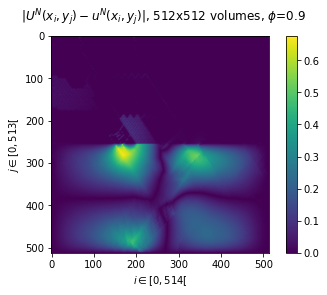
\includegraphics[width=7.5cm]{Images/bicouche/0.9/Figure 2021-11-18 231238 (57).png}
    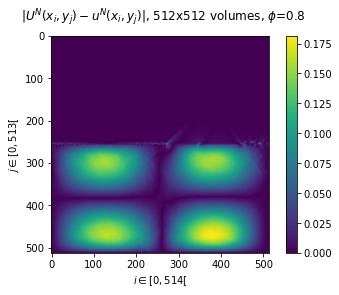
\includegraphics[width=7.5cm]{Images/bicouche/0.8/Figure 2021-11-18 231238 (49).png}
    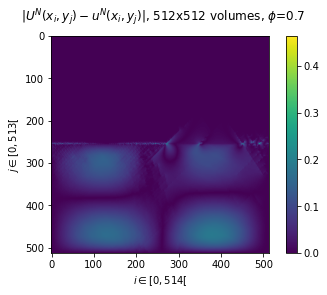
\includegraphics[width=7.5cm]{Images/bicouche/0.7/Figure 2021-11-18 231238 (41).png}
    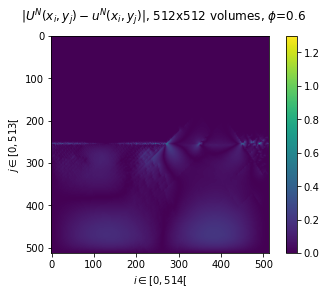
\includegraphics[width=7.5cm]{Images/bicouche/0.6/Figure 2021-11-18 231238 (33).png}
    \caption{Champ d'erreur pour la variable $U_h$}
\end{figure}

\begin{figure}[htp]
    \centering
    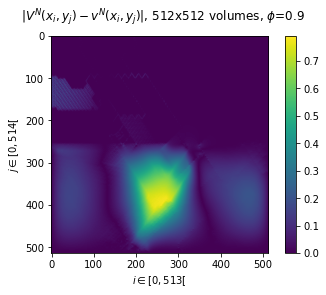
\includegraphics[width=7.5cm]{Images/bicouche/0.9/Figure 2021-11-18 231238 (58).png}
    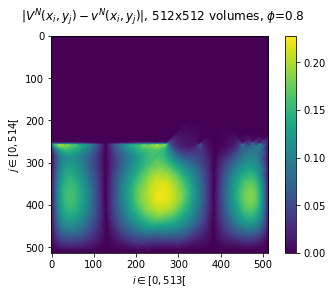
\includegraphics[width=7.5cm]{Images/bicouche/0.8/Figure 2021-11-18 231238 (50).png}
    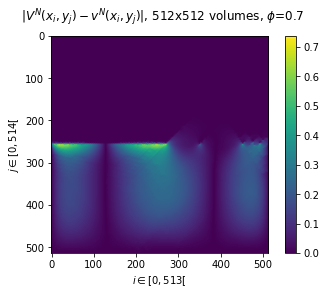
\includegraphics[width=7.5cm]{Images/bicouche/0.7/Figure 2021-11-18 231238 (42).png}
    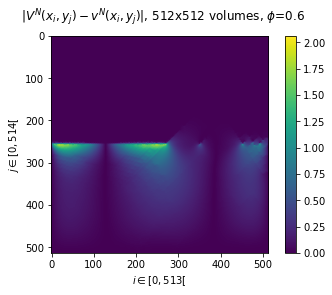
\includegraphics[width=7.5cm]{Images/bicouche/0.6/Figure 2021-11-18 231238 (34).png}
    \caption{Champ d'erreur pour la variable $V_h$}
\end{figure}

\begin{figure}[htp]
    \centering
    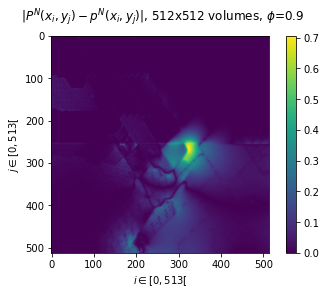
\includegraphics[width=7.5cm]{Images/bicouche/0.9/Figure 2021-11-18 231238 (59).png}
    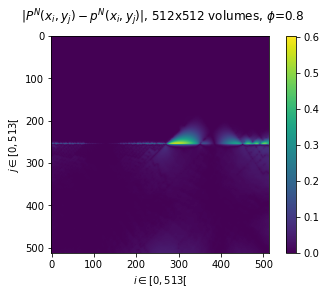
\includegraphics[width=7.5cm]{Images/bicouche/0.8/Figure 2021-11-18 231238 (51).png}
    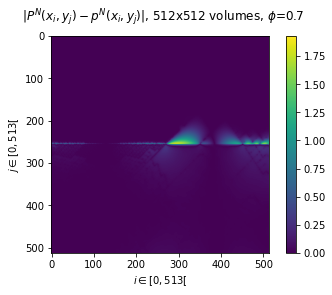
\includegraphics[width=7.5cm]{Images/bicouche/0.7/Figure 2021-11-18 231238 (43).png}
    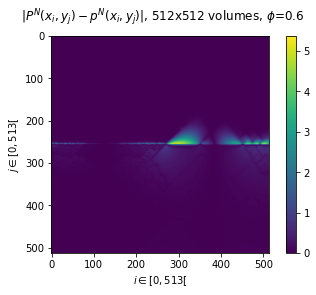
\includegraphics[width=7.5cm]{Images/bicouche/0.6/Figure 2021-11-18 231238 (35).png}
    \caption{Champ d'erreur pour la variable $P_h$}
\end{figure}

On présente enfin les graphes d'analyse.
\begin{figure}[htp]
    \centering
    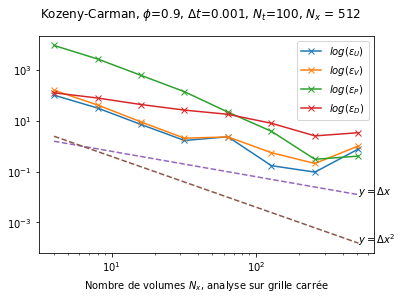
\includegraphics[width=7.5cm]{Images/bicouche/0.9/Figure 2021-11-18 231238 (60).png}
    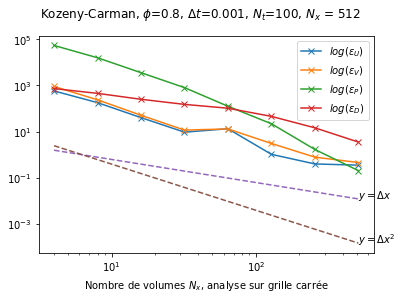
\includegraphics[width=7.5cm]{Images/bicouche/0.8/Figure 2021-11-18 231238 (52).png}
    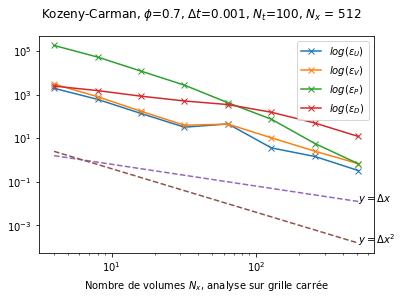
\includegraphics[width=7.5cm]{Images/bicouche/0.7/Figure 2021-11-18 231238 (44).png}
    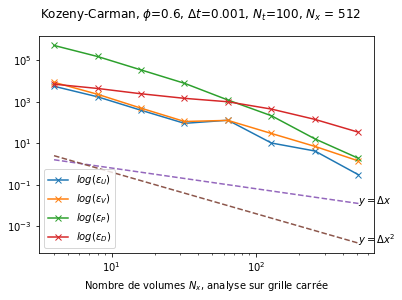
\includegraphics[width=7.5cm]{Images/bicouche/0.6/Figure 2021-11-18 231238 (36).png}
    \caption{Analyse des graphes}
\end{figure}

Bien que les courbes soient cassées, et présentant des valeurs bien trop grandes pour valider le code utilisé, les courbes de vitesse et de pression ont une tendance à l'ordre deux. Le problème réside probablement dans la composition du problème modèle et dans les choix tels que l'emplacement de la surface $\Sigma$.

\section{Conclusion}

Il n'y a pas grand chose à conclure de cette partie si ce n'est que si l'intention était là, le résultat est décevant. Bien sûr, avec plus de temps et de résultat, on aurait voulu poursuivre cette étude en proposant d'autres lois d'une part et un raffinement pour les grandes valeurs de porosité $\phi$. En ce qui concerne l'emplacement de $\Sigma$, il est probable que l'imposer sur une ligne de points de pression est peu astucieux, surtout en vue d'évolutions avec traitement d'un saut non-nul. En effet, la discrétisation de l'opérateur fait intervenir deux valeurs $P^p$ et $P^f$, laquelle doit être imposée sur la ligne en question ?

Autant de questions qui concluent mon mémoire.